\documentclass[usenames,dvipsnames,10pt,aspectratio=169]{beamer} 

\usepackage[utf8]{inputenc}
\usepackage{verbatim}
\usepackage{minted}
\usepackage{graphicx}
\usepackage{wrapfig}
\usepackage{geometry}
\usepackage{listings}
% \usepackage{showframe}
\usepackage{enumitem}
\usepackage{color, xcolor}
\usepackage[document]{ragged2e}
\usetheme{umu}

\usemintedstyle{monokai}

\usepackage{hyperref}
\hypersetup{
    colorlinks=true,
    linkcolor=ucugreyish,
    filecolor=ucured,
    urlcolor=ucublue,
}
\urlstyle{same}

\addtobeamertemplate{navigation symbols}{}{%
    \usebeamerfont{footline}%
    \usebeamercolor[fg]{footline}%
    \hspace{1em}%
    \insertframenumber/\inserttotalframenumber
}
%%% Some useful commands
% pdf-friendly newline in links
\newcommand{\pdfnewline}{\texorpdfstring{\newline}{ }} 
% Fill the vertical space in a slide (to put text at the bottom)
\newcommand{\framefill}{\vskip 0pt plus 1 filll}

%%% Enter additional packages below (or above, I can't stop you)! / Jesper
\renewcommand{\proofname}{\sffamily{Proof}}

% custom fullpage image:
% { % all template changes are local to this group.
%     \setbeamertemplate{navigation symbols}{}
%     \begin{frame}<article:0>[plain]
%         \begin{tikzpicture}[remember picture,overlay]
%             \node[at=(current page.center)] {
%                 
\includegraphics[width=\paperwidth,height=\paperheight]{graphics/version-control.png}
%             };
%         \end{tikzpicture}
%      \end{frame}
% }

% custom shell example inplace
% [fragile] frame
% \begin{lstlisting}[language=Bash, style=shellstyle] 
%     username $ echo a
% \end{lstlisting}

% custom code file
% [fragile] frame
% \lstinputlisting[language=Python, style=codestyle]{code/shebang_ex.py}

% presentation template slides usage
% \framecard[color (not working)]{textbuf}
% \framesplit{Header}{picture}{textbuf}
% \framepic{image}{text}
% \lstinputlisting[language=Bash, style=codestyle]{code/namespace_ex.sh}

%%%%%%%%%%%%%%%%%%%%%%%%%%%%%%%%%%%%%%%%%%%%%%%%%%%%%%%%%%%%%%%%%%%%%%%%%%%%%%%%%%%%%
\title{Linux course}
\subtitle{Processes}
\date[\today]{\small\today}
\author[Morhunenko Mykola]{Morhunenko Mykola}
\institute{APPS@UCU}

\setlist[itemize, 1]{label=$\color{ucublue} \bullet$, leftmargin=-2mm}

\begin{document}

\begin{frame}[noframenumbering]
\titlepage
\end{frame}

\begin{frame}{\contentsname}
    \setbeamercolor{background canvas}{bg=ucugrey}
    \tableofcontents
\end{frame}

\section{Processes. Introduction. General knowlage}
\framecard{Processes. Introduction}
\begin{frame}
    \frametitle{Process}
    \begin{itemize}
        \item What is the difference between the program and the process?
        \item \ex{Program}- a file, containing some information that describes how to construct a process in a runtime
        \item It includes:
        \item Binary format identification - some metainformation about the format of executable file. Nowedays UNIX executable files called\ex{Executable and Linking format (ELF)}
        \item Machine-language instructions - main algorithm of the program
        \item Program entry-point address
        \item Data
        \item Symbol and relocation tables
        \item Some other information, more about that on the\ex[ucublue]{Operating systems course}
        \item In our case -\ex{process}- a program loaded to a memory for execution, with all it's allocated resources
    \end{itemize}
\end{frame}

\begin{frame}[fragile]
    \frametitle{Memory layout of the process (recall PoCO)}
    \begin{itemize}
        \item For each process there is some amount of allocated memory
        \item Usually it reffere to a segments
        \item There are such segments as:
        \begin{itemize}
            \item -\ex{Text segmend}- read only (so the\ex[ucuyellow]{process can not modify it's own code}) shareble (\ex[ucuyellow]{multiple processes can share same executable code}) segment with machine code instructions to the program executing 
            \item -\ex{Initialised data segment} - contains initialised global and static variables
            \item -\ex{Uninitialised data segment}-\ex[ucured]{bss}- contains uninitialised global and static variables. When the program is stored on a disk, space for this segment is not initialised, this space is allocated by the program loader at the beginning of the runtime
            \item -\ex{Heap} - memory area from which memory for variables can be allocated during the runtime
            \item -\ex{Stack} - dynamicly growing area for local variables storage, divided on stack frames. Each stack frame is allocated for each currently called function and stores it's arguments, local variables, return address and return value
        \end{itemize}
        \begin{lstlisting}[language=Bash, style=shellstyle] 
username $ size /bin/ls # check size of a binary file segments
  text    data     bss     dec     hex filename
132378    4840    4824  142042   22ada /bin/ls
\end{lstlisting}
    \end{itemize}
\end{frame}


\framesplitc{Virtual memory (recall PoCO)}{graphics/memory_layout.png}{
    \begin{itemize}
        \item All previocly discussed layout is a layout in a\ex{virtual memory}
        \item As all modern OS's nowedays, Linux kernel do a virtual memory management
        \item The aim of this apprach - to increase efficiency of RAM-CPU communication
        \item \ex{Page}- the smallest fixed-size unit of a virtual memory. In most cases on modern OS's it's size is \ex{4KiB}
        \item \ex{Page table}- one more abstruction close-related to processes. Each process has it's own page table of contents
    \end{itemize}
    \ex[ucuyellow]{\footnotesize Virtual memory scheme for one process on Linux x86-32 is shown on the slide}
}

\framesplitc{Virtual memory (recall PoCO)}{graphics/pages.png}{
    \begin{itemize}
        \item Just to clear things up:
        \item \ex{MMU - memory management unit -}hardware component to manage all cpu-memory communication and caching
        \item \ex{OS memory management - }ensures the availability of memory resources for each process continuously
    \end{itemize}
}

\framesplit{Why do we need virtual memory}{graphics/virtual.jpg}{
    Virtual memory is used for:
    \begin{itemize}
        \item \ex[ucuyellow]{Abstraction} - to be free from physical memory addresses/limits
        \item \ex[ucuyellow]{Processes isolation} - every process in a separate address space
        \item \ex[ucuyellow]{Sharing} - a single mapping can serve multiple needs
        \item \ex[ucuyellow]{Flexibility} - assign a virtual address to a file
    \end{itemize}
}

\framepic{graphics/vm.png}{}

\section{Process states}

\begin{frame}
    \frametitle{Process states}
    \begin{itemize}
        \item As a process executes it changes state according to its circumstances
        \item There are following states in Linux:
        \begin{itemize}
            \item -\ex{CREATED}
            \item -\ex[ucuyellow]{RUNNING \& RUNNABLE} - running or ready to run
            \item -\ex{Waiting}- The process is waiting for an event or for a resource
            \item -\ex[ucuyellow]{INTERRUPTABLE\_SLEEP}- waiting but can be interrupted by signals
            \item -\ex[ucuyellow]{UNINTERRUPTABLE\_SLEEP}- waiting and can not be interrupted under any circumstances
            \item -\ex[ucuyellow]{STOPED}- stopped, usually by receiving a signal
            \item -\ex[ucuyellow]{ZOMBIE}- process that should be terminated, but for some reason (usually some bug) it can not be terminated properly
        \end{itemize}
        \item It is more important for scedualing
    \end{itemize}
\end{frame}

% https://cloudchef.medium.com/linux-process-states-and-signals-a967d18fab64
{ % all template changes are local to this group.
    \setbeamertemplate{navigation symbols}{}
    \begin{frame}<article:0>[plain]
        \begin{tikzpicture}[remember picture,overlay]
            \node[at=(current page.center)] {
                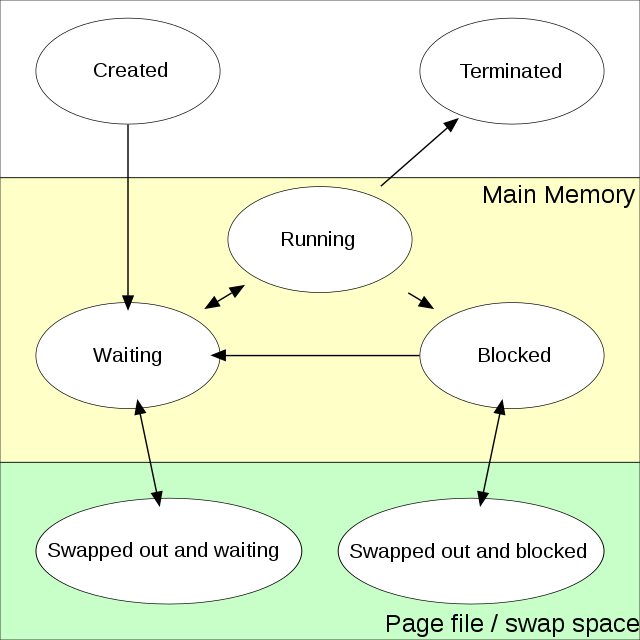
\includegraphics[width=\paperwidth,height=\paperheight]{graphics/states.png}
            };
        \end{tikzpicture}
     \end{frame}
}

\section{Processes Identifiers}

\framepic{graphics/identification.png}{\hspace{250pt} Process \newline \hspace{250pt} Identifiers}

\begin{frame}
    \frametitle{top}
    \begin{itemize}
        \item \ex{top}- program for system monitoring that is part of every Linux system
        \item \ex{htop},\ex{gtop},\ex{ytop},\ex{utop} and othe system monitors may be easier to understand for begginers, but all of them are based on\ex{top}, or inspired by it
        \item Here you can see almost all necessary information about your system and (what is more important) processes
        \item As all other high-performance software, entry bound for this application is too high
        \item Let's see, what is so important information about process can be found in\ex{top}output
    \end{itemize}
\end{frame}

\begin{frame}[fragile]
    \frametitle{PID}
    \begin{itemize}
        \item The very first thing, that is assosiated with any process, it's\ex{PID} - process id 
        \item It's a positive integer, and system works with processes by their PID's - names (commands) are for humans 
        \item There are no fixed ID's for any process, with exception of\ex{init}(more about that in the next topic). PID for\ex{init}equals 1
        \item Maximum PID number for your OS can be found using the following command:
        \begin{lstlisting}[language=Bash, style=shellstyle] 
username $ cat /proc/sys/kernel/pid_max\end{lstlisting}
        \item Also one more important PID for all processes - parrent PID or PPID
        \item If parrent of any process "died" - the child become "adopted" by the\ex{init}process
        \item Parent of any process can be found like:
        \begin{lstlisting}[language=Bash, style=shellstyle] 
username $ cat /proc/PID/status | grep PPid \end{lstlisting}
    \end{itemize}
\end{frame}

\framesplit{Other ID's}{graphics/id.jpg}{
    \begin{itemize}
        \item \ex{UID},\ex{GID}- also ID's that are related to the process, with \ex{RUID (Real User Id)},\ex{SUID (Saved User Id)}and\ex{EUID (Effective User Id)}
        \item In terms of this course it is not important, it is more related to the Linux administration
    \end{itemize}
}

\begin{frame}
    \frametitle{Linux Memory Types}
    \begin{itemize}
        \item There are three main "memory types" in a processes administration
        \item \ex{The physical memory}, limited resource
        \item \ex{Virtual memory}, nearly unlimited resource
        \item \ex{Swap} (optional)
        \item If there is no\ex{swap}on the system, everything will be Ok, up to some point in time (but it is better to have it, and as partition, not as a file)
    \end{itemize}
    

\end{frame}


\section{Scedualing}

\section{Real time processes}

\section{Sources}
\framecard{Sources}
\begin{frame}{Sources}
    \begin{itemize}
        \item \href{https://tldp.org/LDP/tlk/tlk-toc.html}{"The Linux Kernel book", David A Rusling}
        \item "Linux programming interfaces", M. Kerrisk
        \item \href{https://cloudchef.medium.com/linux-process-states-and-signals-a967d18fab64}{Linux process states and signals, Medium(Cloud Chef)}
        \item \href{https://man7.org/linux/man-pages/man1/top.1.html}{top manual}
    \end{itemize}
\end{frame}

\end{document}